\documentclass[pscyr]{hedwork}
\usepackage[russian]{babel}
\usepackage[utf8]{inputenc}
\usepackage{hedmaths}
\usepackage{graphicx}
\graphicspath{{images/}}

\faculty{Факультет электроники и вычислительной техники}
\department{физики}
\subject{Термодинамика и статистическая физика}
\variant{17}
\student[f]{студентка группы Ф-469\\Слоква В. И.}
\teacher[m]{профессор,\\доктор физ.-мат. наук\\Крючков С. В.}

\begin{document}
\maketitle

%-------------------------------------------------------------------------------

\emph{2.41: атмосферное давление изменилось от \( p_1 = 983 \)~гПа до
\( p_2 = 1003 \)~гПа. Какое приращение \( \Delta U \) получает при этом
внутренняя энергия воздуха, содержащегося в комнате объема
\( V = 50,\!0 \text{ м}^3\)? Температура в комнате предполагается неизменной.}

\vspace*{2em}
\emph{Решение:}

запишем выражение для внутренней энергии через теплоемкость при постоянном
объеме~\( C_V \): \( U = C_V \nu T = \dfrac{R}{\gamma - 1}\cdot\nu T \). Для
двухатомного газа \( \gamma = 7/5 \).

Приращение внутренней энергии:
\[
  \Delta U = U_2 - U_1 = \frac{R}{\gamma - 1}\cdot T\big( \nu_2 - \nu_1 \big).
\]

По закону Менделеева-Клапейрона \( \nu = \dfrac{pV}{RT} \), тогда
\[
  \Delta U = \frac{R}{\gamma - 1}\cdot T\left( \frac{p_2V}{RT} -
  \frac{p_1V}{RT} \right) = \frac{V}{\gamma - 1}\big( p_2 - p_1 \big).
\]

Подставим значения:
\[
  \Delta U = \frac{50,\!0 \text{ м}^3}{7/5 - 1}\cdot 20 \text{ гПа} =
  0,\!25 \text{ МДж}.
\]

\vspace*{2em}
\emph{Ответ:} \( \Delta U = 0,\!25\)~МДж.

\newpage %----------------------------------------------------------------------

\emph{2.65: некоторое количество идеального газа (\( \gamma = 1,\!40 \))
расширяется от \( V_1 = 20,\!0 \)~л до \( V_2 = 50,\!0 \)~л так, что процесс на
диаграмме \( (p, V) \) имеет вид прямой линии. Исходное давление
\( p_1 = 1000 \)~гПа, конечное \( p_2 = 2000 \)~гПа.\\
а) Является ли процесс политропическим?\\
б) Найти количество теплоты \( Q \), поглощаемое газом в ходе расширения.}

\vspace*{2em}
\emph{Решение:}

\begin{table}[ht]
  \center
  \begin{tabular}{m{.6\textwidth}@{\hspace{2em}}C{.4}}
    по определению политропического процесса:
    \[
      PV^n = \const
    \]
    Из графика видно, что \( p = aV \), где
    \[
      a = \tg\alpha = \dfrac{p_2 - p_1}{V_2 - V_1}.
    \]
    
    Уравнение политропического процесса преобразуется к виду
    \( aV^{n + 1} = \const \) и
    \[
      aV_1^{n+1} = aV_2^{n+1}, \qquad \left( \frac{V_1}{V_2} \right)^{n+1} = 1.
    \]
    & 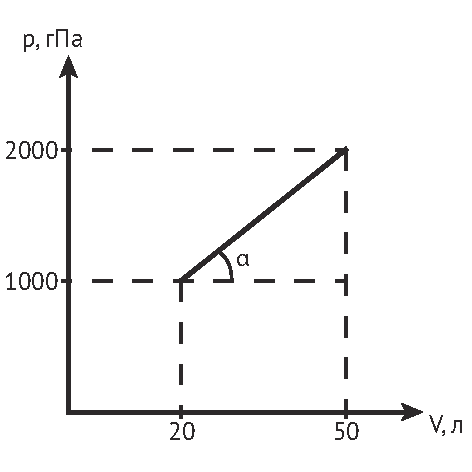
\includegraphics[width=.4\textwidth]{2_65}
  \end{tabular}
\end{table} \vspace{-2em}
Отсюда \( n = -1 \) и \( \dfrac{p}{V} = \const \).

Таким образом процесс является политропическим с \( n = - 1 \).\\

По первому началу термодинамики: \( Q = \Delta U + A \).

Запишем выражение для внутренней энергии через теплоемкость при постоянном
объеме~\( C_V \): \( \Delta U = C_V\Delta T = \dfrac{R}{\gamma - 1}\cdot
(T_2 - T_1) \).

По закону Менделеева-Клапейрона \( T = \dfrac{pV}{R} \), тогда \( \Delta U \):
\[
  \Delta U = \frac{R}{\gamma - 1}\cdot\frac{p_2V_2 - p_1V_1}{R} =
  \frac{p_2V_2 - p_1V_1}{\gamma - 1} = 20\text{ кДж}.
\]

Работа, по определению,
\[
  A = \int\limits_{V_1}^{V_2} p\,dV = a\int\limits_{V_1}^{V_2} V\,dV =
  \frac{p_2 - p_1}{V_2 - V_1}\cdot\frac{V_2^2 - V_1^2}{2} = 4,\!5\text{ кДж}.
\]

Тогда количество тепла \( Q = \Delta U + A =  24,\!5 \)~кДж.

\vspace*{2em}
\emph{Ответ:} а) да, \( n = -1 \); б) \( Q = 24,\!5\)~кДж.

\newpage %----------------------------------------------------------------------

\emph{2.96: вблизи поверхности Земли отношение объемных концентраций кислорода
(\( O_2 \)) и азота (\( N_2 \)) в воздухе \( \eta_0 = 20,\!95/78,\!08 =
0,\!268 \). Полагая температуру атмосферы не зависящей от высоты и равной
\( 0^\circ C \), определить это отношение \( \eta \) на высоте \( h = 10 \)~км.}

\vspace*{2em}
\emph{Решение:}

по барометрической формуле:
\[
  \eta\big(h\big) = \eta_0\cdot\exp\left(-mg\cdot\frac{h - h_0}{RT}\right),
\]
где \( m = M_{O_2} + M_{N_2} \).

Подставим числовые значения:
\[
  \eta\big(10\text{ км}\big) = 0,\!268\cdot\exp\left(-\frac{(32 + 28)\cdot
  9,\!8\cdot10^{4}}{8,\!31\cdot273}\right) = 0,\!225.
\]

\vspace*{2em}
\emph{Ответ:} \( \eta\big(10\text{ км}\big) = 0,\!225 \).

\newpage %----------------------------------------------------------------------

\emph{2.132: найти приращение энтропии \( \Delta S \) при конденсации массы
\( m = 1,\!00 \)~кг пара, находившегося при температуре \( t_1 = 100^\circ C \),
в воду и последующем охлаждении до температуры \( t_2 = 20^\circ C \).
Теплоемкость воды считать не зависящей от температуры. Конденсация происходит
при давлении, равном 1~атм.}

\vspace*{2em}
\emph{Решение:}

изменение энтропии есть разница энтропий двух состояний:
\[
  \Delta S = S_2 - S_1 = \int\limits_1^2 \frac{\delta Q}{T} =
  \frac{\delta Q_2}{T} - \frac{\delta Q_1}{T},
\]
где \( \displaystyle \delta Q_2 = \int\limits_{T_1}^{T_2} cm\,dT \), \quad
\( \delta Q_1 = mq_\text{п} \), \( q_\text{п} \) -- удельная теплота
парообразования.

Таким образом,
\[
  \Delta S = \int\limits_{T_1}^{T_2} cm\frac{dT}{T} - \frac{mq_\text{п}}{T_1} =
  m\big(c\ln(T_2/T_1) - q_\text{п}/T_1\big).
\]

Подставим значения:
\[
  \Delta S = 1\text{ кг}\cdot
  \left( 4200\,\frac{\text{Дж}}{\text{кг}\cdot\text{К}} \cdot
  \ln\big( 293/373 \big) - \frac{2,\!3\cdot 10^6}{373}
  \frac{\text{Дж}}{\text{кг}\cdot\text{К}} \right)
  \approx -7 \text{ кДж}/\text{К}.
\]

\vspace*{2em}
\emph{Ответ:} \( \Delta S = -7 \) кДж/К.

\newpage %----------------------------------------------------------------------

\emph{204: В цикле Карно в качестве холодильника выбрана вода при \( 4^\circ\)C.
Так как температурный коэффициент расширения при этой температуре равен нулю, то
для осуществления цикла Карно не надо сообщать тепло холодильнику, т.~е. КПД
цикла равен единице. В чем ошибочность этого рассуждения?}

\vspace*{2em}
\emph{Решение:}
\begin{enumerate}
  \item пусть во всех точках изотермы
  \( \displaystyle \left( \pder{V}{T} \right)_P = 0 \). Тогда
  \( \displaystyle \left( \pder{P}{T} \right)_V = 0 \), и
  \[
    dU = \left[ T\left(\pder{P}{T}\right)V - P \right]dV = -P\,dV.
  \]

  По первому началу термодинамики:
  \[
    \delta Q = dU + P\,dV = -P\,dV + P\,dV = 0.
  \]

  Таким образом, изотерма во всех точках должна совпадать с адиабатой. В этом
  случае цикл Карно между температурой \( 4^\circ\)C и какой-либо другой
  неосуществим.
  \item Для воды коэффициент теплового расширения обращается в нуль только в
  одной точке изотермы, так что условия задачи неосуществимы.
\end{enumerate}

\newpage %----------------------------------------------------------------------

\emph{306: Импульс фотона связан с его энергией соотношением \( \eps = pc \).
Написать выражение для давления \( P \) фотонного газа.}

\vspace*{2em}
\emph{Решение:}

в общем виде давление газа имеет вид:
\[
  P = \sum n_iv_{iz}p_{iz}.
\]

Усредним значение \( v_{z}p_{z} \):
\[
  \average{v_zp_z} = \frac{1}{n}\sum n_iv_{iz}p_{iz}.
\]

Тогда давление примет вид \( P = n\average{v_zp_z} \). По определению скалярного
произведения
\[
  \average{vp} = \average{v_xp_x} + \average{v_yp_y} + \average{v_zp_z}.
\]

Так как направления скоростей равнозначны, то
\[
  \average{v_xp_x} = \average{v_yp_y} = \average{v_zp_z} =
    \frac{1}{3}\average{vp}.
\]

Таким образом, давление примет вид \( P = n\average{vp}/3 \).

Если объем сосуда, в котором заключен газ, равен \( V \), а полное число фотонов
равно \( N \), то \( n = N/V \), и тогда:
\[
  P = \frac{N}{3V}\average{vp}, \text{ или }
    PV = \frac{1}{3}\average{Nvp}.
\]

По условию, \( v = c \), \( p = \eps/c \):
\[
  PV = \frac{1}{3}\average{Ncp} = \frac{1}{3}\average{N\eps} =
    \frac{1}{3}\average{E},
\]
где \( \average{E} \)~-- средняя полная энергия фотонов в сосуде.

\vspace*{2em}
\emph{Ответ:} \( P = 1/3\average{E} \).

\newpage %----------------------------------------------------------------------

\emph{455: Ниже приведены значения постоянных Ван-дер-Ваальса для некоторых
газов:}
\begin{table}[ht]
  \center
  \begin{tabular}{|l|*{2}{C{.3}|}} \hline
    Газ & \( a, 10^6 \text{ атм}\cdot\text{см}^6/\text{моль}^2 \) &
      \( b, \text{см}^2/\text{моль} \) \\ \hline
          Гелий & 0,034 & 23,7 \\
        Водород &  0,24 & 26,6 \\
           Азот &  1,39 & 39,1 \\
       Кислород &  1,36 & 31,8 \\
     CO\( _2 \) &  3,60 & 42,7 \\ \hline
  \end{tabular}
\end{table}
\emph{Пользуясь этими значениями, вычислить критическое давление, критическую
температуру, критический объем, а также температуру Бойля для приведенных газов
в предположении, что они подчиняются уравнению Ван-дер-Ваальса.}

\vspace*{2em}
\emph{Решение:}

для газов, подчиняющихся уравнению Ван-дер-Ваальса, температура Бойля и
критические значения давления, объема, температуры выглядят следующим образом:
\[
  T_B = \frac{a}{bR}, \quad
  P_\text{к} = \frac{a}{27b^2}, \quad
  V_\text{к} = 3b, \quad
  T_\text{к} = \frac{8}{27}\frac{a}{bR}.
\]

Подставляя значения \( a \) и \( b \), получим:
\begin{table}[ht]
  \center
  \begin{tabular}{|l|*{4}{C{.1}|}} \hline
    Газ & \( V_\text{к}, \text{ см}^3 \) & \( P_\text{к} \), атм &
      \( T_\text{к} \), К & \( T_B \), К \\ \hline
          Гелий &  71,1 &  2,24 &   5,18 &   17,5 \\
        Водород &  79,8 & 12,56 &  32,58 &  110,0 \\
           Азот & 117,3 & 33,67 & 128,36 &  433,2 \\
       Кислород &  95,4 & 49,81 & 154,43 &  521,2 \\
     CO\( _2 \) & 128,1 & 73,13 & 304,43 & 1027,4 \\ \hline
  \end{tabular}
\end{table}
\end{document}
